\documentclass[12pt]{article}
\usepackage{blindtext}
\usepackage[utf8]{inputenc}
\usepackage{listings}
\usepackage{mathtools}
\usepackage{graphicx}
\usepackage{matlab-prettifier}
\usepackage{subcaption}
\usepackage[margin=1.3in]{geometry}
\addtolength{\topmargin}{-.5in}
\linespread{1}
\usepackage{setspace}
\usepackage{fancybox}
\usepackage{amsmath}% http://ctan.org/pkg/amsmath
\usepackage{array}
\usepackage{tabu}
\usepackage{bm}
\setlength{\parindent}{0pt}
\bibliographystyle{IEEEtran}


\definecolor{grey}{rgb}{0.9,0.9,0.9} % Color of the box surrounding the title - these values can be changed to give the box a different color	

\thispagestyle{empty}

\date{16 March 2017}
 
\begin{document}
\vspace*{6cm}
\colorbox{white}{
	\parbox[t]{1.0\linewidth}{
		\centering \fontsize{50pt}{80pt}\selectfont % The first argument for fontsize is the font size of the text and the second is the line spacing - you may need to play with these for your particular title
		\vspace*{0.7cm} % Space between the start of the title and the top of the grey box
		
		{401I - Final Year Project} \break
		\vspace*{0.7cm}
		Interim Report
		\break
		Voice Recognition RPG
		\break
		Baron Khan (bak14)
		\vspace*{0.7cm} % Space between the end of the title and the bottom of the grey box
	}
}
\vfill % Space between the title box and author information




\newpage
\setcounter{page}{1}
\section{Introduction}
In recent years, video games have explored various forms of input that diverge from the traditional control schemes of a keyboard and mouse, or an analogue stick and buttons on a controller. Touch-screen controls and motion controls have had varying degrees of success over the years, and provide new forms of interactions with games. A recent form of input used in video games has been voice controls; a user speaks a sentence or phrase and this would execute an action or intent within the game.
\\
\\
Voice recognition and control schemes have been used in various ways in the medium, whether in tandem with traditional control schemes, or as the only form of input. The hardware running the game requires a microphone that always listens to the user (or detects a 'hot-word' phrase in order to begin accepting voice input), whether this is built into the hardware architecture, or external hardware connected to the main system. The audio input requires some pre-processing (e.g. noise-filtering, de-reverberation, echo cancellation, etc.) before it can be intelligible and used in the game.
\\
\\
Most games which feature a voice control scheme are typically programmed to work with a specific set of keywords or phrases, hard-coded by the developer. The is usually the case with games where the voice control interface is entirely optional to use, as it requires little to no input from the programmer; if the speech processing is handled by a separate library, the developer just has to map a text string (e.g. "open the door") to the function that executes the intent (e.g. the function that opens a nearby door in the game).
\\
\\
It becomes increasingly difficult for the developer to add more phrases that can be accepted in the game and map to the same intent (e.g. "push the door open") as they would have to hard-code each possible input that the user could possibly say: having too few phrases would mean that the user could become frustrated when their preferred way of stating an intent is not accepted by the game, while adding too many acceptable phrases would increase development time.
\\
\\
Natural Language Processing (NLP, also referred to as Natural Language Understanding) has been used to improve inference of what users were trying to say, and to extract meaning from the user's phrases and sentences. For instance, if the user says, "push the door open", NLP can be used to infer that the user's intent is to open a door. Using NLP, several user phrases can be mapped to the same intent without having to hard-code each possible phrase.
\\
\\
NLP is already used to improve voice recognition in popular personal assistants such as Siri, but these systems offload the NLP workload to the server to reduce the amount of local processing required, as NLP requires a sizeable amount of machine learning and pattern recognition \cite{RefWorks:21}.
\\
\\
The goal of this project is to apply NLP to a voice control scheme used within a role-playing game (RPG), in order to reduce the amount of work required by a developer to add a flexible voice control interface, and to give more freedom of expression to the player while they play the game.
\\
\\
Role-playing games involve the player controlling a character in a world featuring exploration and/or battle mechanics, along with a progression system, where the character gains new abilities as the game progresses. These include turn-based games such as Pokemon and Final Fantasy, or more action-based games such as Dark Souls or Skyrim. In these games, the player possesses several items that they acquire during the game, and accesses them by navigating menus.
\\
\\
If the player has many different items, they may need to spend a lot of time searching the menus for a specific item, which can be quite tedious. It can also become quite repetitive if the user is constantly only pushing the "Attack" button over and over again with no variation in the attack used. Using voice recognition and NLP, a player could just simply say a phrase such as, "use a potion" or, "attack with axe", and the corresponding item will be used without having the player navigate several menu screens.
\\
\\
A simple mobile RPG will be created that will use a flexible voice control interface. It will feature a simple exploration mechanic, with the user manipulating objects and environments with commands, and a simple battle mechanic. These will be designed to fully demonstrate the power of the voice-control system to make the game easier to play, as opposed to using traditional mouse clicks and button presses. The target platform will be Android phones to allow for hand-free voice control input.

\newpage
\section{Background}
\subsection{Voice Control in Games}
Below is a list of notable recent games that have incorporated voice control functionality as a major component of the interaction experience.
\subsubsection{In Verbis Virtus}
In Verbis Virtus \cite{RefWorks:22} is an independent 3D fantasy adventure game developed by Indomitus Games for Windows. It requires the player to solve puzzles in a 3D environment and battle enemies using magic.
\\
\\
When a microphone is connected, the player is able to cast spells using their voice by saying specific phrases defined by the game. For example, to cast a spell that produces a floating light source to brighten a room, a user must say, "let there be light", or if the user wishes to shoot an energy beam from their hand, they must say, "Beam of Light", and so. These phrases appear to be hard-coded into the game.
\\
\\
There are several limitations with this implementation of voice control. Firstly, since the phrases are hard-coded, there is no lenience in variations of the phrases, e.g. "create a light" or "Laser of Light", etc. This can seem mundane and no different to a user pressing the same button repeatedly to cast a spell.
\\
\\
Another limitation is that the user is still required to use a keyboard and mouse to perform other actions in the game, such as moving around, looking around, and navigating menus and message boxes. The voice control interface cannot be used to perform these actions. The voice control interface itself does not seem integral to the experience, as the user could just simply press a key that performs the spell instead of saying the same phrase over and over again.
\\
\\
This voice recognition interface could be improved by allowing the player to perform any action within the game using their voice, as well as allowing for more variation in what the user can say for each action.

\subsubsection{Skyrim Kinect}
The Elders Scrolls V: Skyrim is first-person action role-playing game developed by Bethesda \cite{RefWorks:23}. The Xbox 360 version of the game supports the Microsoft Kinect peripheral which allows the the player to execute voice commands \cite{RefWorks:24}. The user can use over 200 hundred pre-configured voice commands, and these can be used simultaneously with the traditional control scheme.
\begin{center}
\begin{figure}
  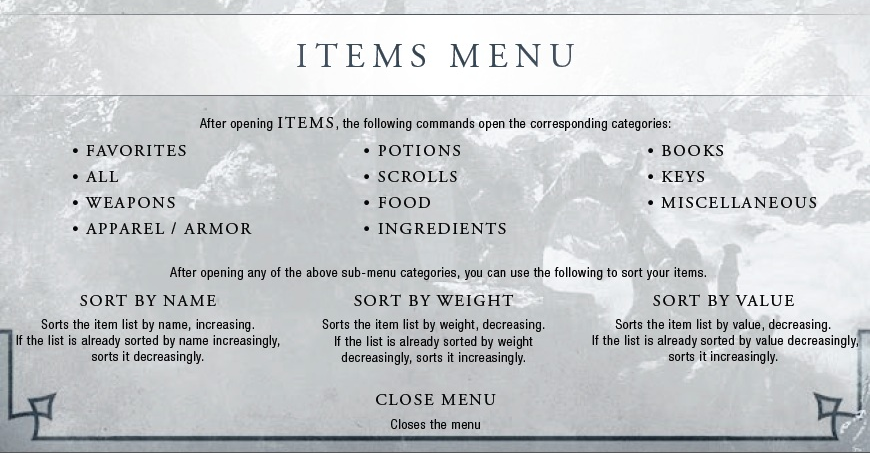
\includegraphics[width=\textwidth]{skyrim-item-commands.png}
  \caption{Voice commands that are available within the items menu in Skyrim.}
\end{figure}
\end{center}
There are voice commands available that allow the user to navigate the game's menu screens. For instance, the player would say, "quick items" to open their inventory menu. Afterwards, the user can open menus for specific categories of items such as "potions", "books", etc. However, it doesn't seem to be possible to actually use any of the items selected with only voice command from the menu; this is only possible if you assign the item to a 'hotkey' (e.g. by saying, "assign health potion" once you have highlighted a potion item), and then saying "equip health potion" during the game. See the Appendix for a full list of of available voice commands.
\\
\\
This system, despite being optional to the player, helps to reduce the time spent searching through the menu screens. However, this system also hard-codes the phrases that can be said by the player with no flexibility.

\subsubsection{Star Trek Bridge Crew}

Star Trek Bridge Crew is a virtual reality game developed by Ubisoft [5]. This game allows the player to issue voice commands to AI crew members on a spaceship. In order to develop a more interactive and realistic experience, the development team used IBM Watson's interactive speech capabilities. This API allows commands to be delivered in a variety of ways, as the speech is parsed for its meaning using Watson's Conversation service. For example, a player could say, "show me the ship's status report" or they could say something drastically different such as "damage report" to execute the same command. This gives the user more freedom in how they convey their request to the AI. IBM's Watson API is described in more detail in a later section of this report.
\\
\\
The voice recognition design used in this game is similar to the proposed design outlined in this report. The user's intent should be extracted from the phrase that they speak, so similar phrases should map to the same intent. Unfortunately, Watson's API is a paid cloud service; not only does it require a constant internet connection, but users are also charged for each API call they make.

\subsection{Voice Control Implementations}





\newpage
TODO: add brackets around title in bib file.
\bibliography{references}
\end{document}